从道义上讲，一个\trInfinityCosmos{}可以被描述为「一个具备 $(\infty,2)$-范畴论
极限的 $(\infty,2)$-范畴」，但\cref{def:infinity-cosmos}给出的精确公理化对这句话
采用了一种格外严格的解读，借助众多例子中现成的严格性来简化证明。我们把∞-宇宙
定义为以\trQuasiCategory{}富集的范畴——这选取了通行使用中最严格的一种
$(\infty,2)$-范畴模型（见 \cite[0.0.3-4]{bib79}）——并以某些同伦性质良好的%
\trSimpliciallyEnrichedLimit{}来构造 $(\infty,2)$-范畴论极限。

本章的目标是发展出更多的\trInfinityCosmos{}例子；这立即使我们得以把第一部分中
证明的全部定理应用于更为\trExotic{}语境——在这些语境中，一个%
\trInfinityCosmos{}的诸\trInfinityCategory{}不应被设想为「某种模型中的
$(\infty,1)$-范畴」。这些例子中有一些——例如 6.1 节中引入的%
\trIsofibration{}的\trInfinityCosmos——只需直接验证\cref{def:infinity-cosmos}的
公理便可轻松确立。

更大的一族例子出现于 6.3 节，它们作为先前定义的\trInfinityCosmos{}的子范畴而
产生。例如，命题 6.3.14 将证明：任一\trInfinityCosmos{} $\mathcal{K}$ 中%
\trIsofibration{}的\trInfinityCosmos{} $\mathcal{K}^{\dagger}$ 具有一个子∞-宇宙
$\mathcal{C}\mathit{art}(\mathcal{K})$，由\trCartesianFibration{}与其间的笛卡尔
函子组成。
这一结果以及许多类似趣味的结果，都源自一个以命题 6.3.3 出现的共同范式：%
\trInfinityCosmos{}的一个\emph{充盈}（replete）子范畴（见定义 6.3.1），只要对%
\emph{柔性加权极限}（flexible weighted limits）封闭，便继承一个∞-宇宙结构。

这引出本章的第二个主旨：对任一\trInfinityCosmos{}中现存的 $(\infty,2)$-范畴论
极限的细致阐发。在 6.2 节中我们将发现，\cref{def:infinity-cosmos}(i) 所列举的%
\trCosmologicalLimitNotions{}生成一个大得多的\trSimpliciallyEnrichedLimit{}类
——它们存在于任何\trInfinityCosmos{}中，并且恰恰是那些无愧于称作
「$(\infty,2)$-范畴论极限」的\trSimpliciallyEnrichedLimit。我们把这些%
\trSimpliciallyEnrichedLimit{}称为\emph{柔性加权极限}，此语借自 2-范畴论
（见题外话 6.2.7）。

为解释其直观，我们利用富集范畴论中\trWeightedLimit{}的形式化工具（见 A.6 节）。
通常的\trLimit{}对给定的\trDiagram{}定义出一个泛\trCone，锥的每条腿都是以极限
对象为源的一支箭头。\trWeightedLimit{}同样对给定的\trDiagram{}定义泛\trCone，
但此时\trCone{}可以取更为\trExotic{}形状。在单纯富集的语境下，每条锥腿都可以
取任意\trSimplicialSet{}的形状，而锥的交换性条件则由一个取值于单纯集的%
\trSimplicialFunctor{}指定，称为\emph{权}（weight）。例如，\trCospan{}上的
通常\trCone{}定义一个交换方块，而对权的另一种选择，其锥便是内驻有一支
1-\trSimplex{}的方块。定义 3.4.1 的诸\trCommaInfinityCategory{}正是以这种方式
作为\trCospan{}的\trWeightedLimit{}而产生的（见例 A.6.14）。

直观地说，柔性加权极限就是那些权所定义的锥形不施加任何严格交换性条件的%
\trLimit{}：\trPullback{}不是柔性加权极限，而逗号对象则是。柔性加权极限在图表
之间的逐点\trEquivalence{}之下不变，而一般的\trWeightedLimit{}则未必。这正是
柔性加权极限对应于 $(\infty,2)$-范畴论极限概念的两层意义。

在确立柔性加权极限的同伦性质之后，我们还会看到，诸\trCosmologicalLimitNotions{}%
——诸如\trIsofibration{}的\trPullback{}——其实是化了装的柔性加权极限。要求
图表中的某些箭头是\trIsofibration，恰好使得严格交换的锥对应于%
\trPseudoCommutative{}锥，从而提供所需的柔性。

本章最后以若干示例展示这里所发展的一般∞-宇宙论的应用。更多应用将见于第二部分，
我们在那里用本章构造的诸\trInfinityCosmos{}来发展双侧纤维化与模的理论。

\providecommand{\Fun}{\operatorname{Fun}}
\providecommand{\qcOne}{\mathbf{1}}   %
\providecommand{\qcTwo}{\mathbf{2}}   %
\providecommand{\twoheaddownarrow}{\rotatebox[origin=c]{270}{$\twoheadrightarrow$}}   %

\section{等价纤维化的∞-宇宙}\label{sec:isofibration-cosmos}

我们的第一个「\trExotic{}∞-宇宙」的例子，是一个更一般结果的特例，该结果留作%
\cref{ex:inverse-reedy-cosmos}。\trWalkingArrow{}\trCategory{} $\qcTwo$ 是一个%
\emph{逆 Reedy 范畴}（inverse Reedy category），其中非恒同箭头的定义域被指派
次数一、余定义域被指派次数零。这一 Reedy 结构为我们在下文引入的%
\textbf{\trIsofibration{}的\trInfinityCosmos}（∞-cosmos of isofibrations）中的诸定义提供了动机：

\begin{proposition}[等价纤维化的∞-宇宙]\label{prop:isofibration-cosmos}
对任何\trInfinityCosmos{} $\mathcal{K}$，存在一个\trInfinityCosmos{}
$\mathcal{K}^{\dagger}$，使得：
\begin{itemize}
\item[(i)] 其对象是 $\mathcal{K}$ 中的\trIsofibration{}
$p\colon E\twoheadrightarrow B$；
\item[(ii)] 其\trFunctorSpace{}——比如从 $q\colon F\twoheadrightarrow A$ 到
$p\colon E\twoheadrightarrow B$ 的\trFunctorSpace——由\trPullback{}定义
\begin{center}
\begin{tikzpicture}[x=1.15em,y=1.15em]
  \node (TL) at (0,1.7) {$\Fun({F\overset{q}{\twoheadrightarrow}A},{E\overset{p}{\twoheadrightarrow}B})$};
  \node (TR) at (12.4,1.7) {$\Fun(F,E)$};
  \node (BL) at (0,0) {$\Fun(A,B)$};
  \node (BR) at (12.4,0) {$\Fun(F,B)$};
  \draw[->] (7.3,1.7) -- (10.4,1.7);
  \draw[->>] (0,1.2) -- (0,0.5);
  \node at (0.55,1.28) {$\scriptstyle\lrcorner$};
  \draw[->>] (12.4,1.2) -- (12.4,0.5);
  \node at (13.1,0.85) {$\scriptstyle p^{*}$};
  \draw[->] (1.7,0) -- (10.3,0);
  \node at (6.0,-0.45) {$\scriptstyle q^{*}$};
\end{tikzpicture}
\end{center}
\item[(iii)] 从 $q$ 到 $p$ 的\trIsofibration{}是交换方块
\begin{center}
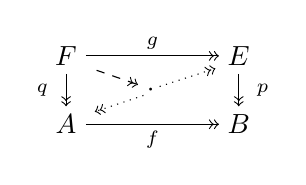
\begin{tikzpicture}[x=1.3em,y=1.3em]
  \node (F) at (0,1.9) {$F$};
  \node (E) at (4.8,1.9) {$E$};
  \node (A) at (0,0) {$A$};
  \node (B) at (4.8,0) {$B$};
  \draw[->>] (0.55,1.9) -- (4.25,1.9);
  \node at (2.4,2.26) {$\scriptstyle g$};
  \draw[->>] (0,1.4) -- (0,0.5);
  \node at (-0.66,0.95) {$\scriptstyle q$};
  \draw[->>] (4.8,1.4) -- (4.8,0.5);
  \node at (5.46,0.95) {$\scriptstyle p$};
  \draw[->>] (0.55,0) -- (4.25,0);
  \node at (2.4,-0.42) {$\scriptstyle f$};
  \node at (2.35,0.95) {$\cdot$};
  \draw[->>,dashed] (0.85,1.5) -- (2.0,1.1);
  \draw[->>,dotted] (2.6,1.05) -- (4.15,1.55);
  \draw[->>,dotted] (2.15,0.8) -- (0.8,0.35);
  \node at (2.75,0.62) {$\scriptstyle\lrcorner$};
\end{tikzpicture}
\end{center}
其中诸水平箭头以及从初始顶点到\trCospan{}之\trPullback{}的诱导映射都是
$\mathcal{K}$ 中的\trIsofibration；
\item[(iv)] \trLimit{}在 $\mathcal{K}$ 中逐点定义；
\item[(v)] 且一个映射
\begin{center}
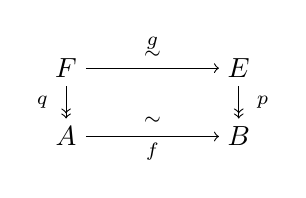
\begin{tikzpicture}[x=1.3em,y=1.3em]
  \node (F) at (0,1.9) {$F$};
  \node (E) at (4.8,1.9) {$E$};
  \node (A) at (0,0) {$A$};
  \node (B) at (4.8,0) {$B$};
  \draw[->] (0.55,1.9) -- (4.25,1.9);
  \node at (2.4,2.6) {$\scriptstyle g$};
  \node at (2.4,2.26) {$\scriptstyle\sim$};
  \draw[->>] (0,1.4) -- (0,0.5);
  \node at (-0.66,0.95) {$\scriptstyle q$};
  \draw[->>] (4.8,1.4) -- (4.8,0.5);
  \node at (5.46,0.95) {$\scriptstyle p$};
  \draw[->] (0.55,0) -- (4.25,0);
  \node at (2.4,0.44) {$\scriptstyle\sim$};
  \node at (2.4,-0.42) {$\scriptstyle f$};
\end{tikzpicture}
\end{center}
是 $\mathcal{K}^{\dagger}$ 中的\trEquivalence，当且仅当 $g$ 与 $f$ 是
$\mathcal{K}$ 中的\trEquivalence。
\end{itemize}
相对于这些定义，定义域\trFunctor、余定义域\trFunctor{}与恒同\trFunctor
\begin{center}
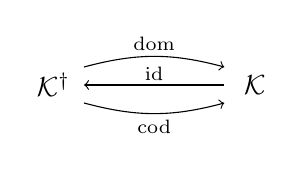
\begin{tikzpicture}[x=1.3em,y=1.3em]
  \node (Kd) at (0,0) {$\mathcal{K}^{\dagger}$};
  \node (K) at (5.6,0) {$\mathcal{K}$};
  \draw[->] (0.85,0.5) to[bend left=15] (4.75,0.5);
  \node at (2.8,1.15) {$\scriptstyle\mathrm{dom}$};
  \draw[->] (4.75,0) -- (0.85,0);
  \node at (2.8,0.32) {$\scriptstyle\mathrm{id}$};
  \draw[->] (0.85,-0.5) to[bend right=15] (4.75,-0.5);
  \node at (2.8,-1.15) {$\scriptstyle\mathrm{cod}$};
\end{tikzpicture}
\end{center}
都是宇宙论的。
\end{proposition}

\begin{proof}
\trDiagram{}\trCategory{} $\mathcal{K}^{\dagger}$ 从 $\mathcal{K}$ 逐点继承其%
\trSimpliciallyEnrichedLimit；(ii) 中描述的\trFunctorSpace{}就是图表之富集范畴
的通常\trFunctorSpace。这就验证了\cref{def:infinity-cosmos}(i)。注意，%
\trFunctorSpace、\trLimit{}与\trIsofibration{}的这些定义使得定义域、余定义域
与恒同\trFunctor{}个个都是宇宙论的。

对于\cref{def:infinity-cosmos}(ii)，注意积\trFunctor{}与%
\trSimplicial\trCotensor{}函子把逐点的\trIsofibration{}送到\trIsofibration。(iii)
中那样的\trIsofibration{}沿一个从\trIsofibration{} $r$ 到 $p$ 的交换方块所作的%
\trPullback{}可以在 $\mathcal{K}$ 中形成。我们的任务是证明诱导映射 $t$ 是%
\trIsofibration，并且从 $t$ 到 $r$ 的方块在 (iii) 的意义下是\trIsofibration：
\begin{rveq}\label{eq:isofibration-pullback}
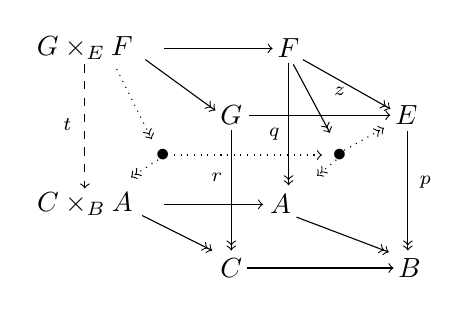
\begin{tikzpicture}[x=1.15em,y=1.15em]
  \node (GEF) at (0,6.9) {$G\times_{E}F$};
  \node (F)   at (6.4,6.9) {$F$};
  \node (G)   at (4.6,4.8) {$G$};
  \node (E)   at (10.1,4.8) {$E$};
  \node (pb1) at (2.45,3.55) {$\bullet$};
  \node (pb2) at (8.0,3.55) {$\bullet$};
  \node (CBA) at (0,2.0) {$C\times_{B}A$};
  \node (A)   at (6.15,2.0) {$A$};
  \node (C)   at (4.6,0) {$C$};
  \node (B)   at (10.2,0) {$B$};
  \draw[->] (2.5,6.9) -- (5.9,6.9);
  \draw[->>] (1.9,6.55) -- (4.1,4.95);
  \draw[->,dashed] (0,6.4) -- (0,2.5);
  \node at (-0.55,4.5) {$\scriptstyle t$};
  \draw[->] (5.15,4.8) -- (9.6,4.8);
  \draw[->>] (6.85,6.55) -- (9.6,5.0);
  \node at (8.0,5.55) {$\scriptstyle z$};
  \draw[->>] (6.55,6.4) -- (7.7,4.25);
  \draw[->>] (6.4,6.45) -- (6.4,2.6);
  \node at (5.95,4.2) {$\scriptstyle q$};
  \draw[->>] (4.6,4.35) -- (4.6,0.55);
  \node at (4.15,2.85) {$\scriptstyle r$};
  \draw[->>] (10.15,4.3) -- (10.15,0.55);
  \node at (10.7,2.7) {$\scriptstyle p$};
  \draw[->] (2.5,2.0) -- (5.6,2.0);
  \draw[->>] (1.8,1.65) -- (4.0,0.55);
  \draw[->>] (6.65,1.6) -- (9.55,0.5);
  \draw[->] (5.1,0) -- (9.7,0);
  \draw[->>,dotted] (1.0,6.25) -- (2.1,4.05);
  \draw[->>,dotted] (2.3,3.4) -- (1.45,2.85);
  \draw[->,dotted] (2.8,3.55) -- (7.45,3.55);
  \draw[->>,dotted] (8.15,3.7) -- (9.4,4.4);
  \draw[->>,dotted] (7.9,3.4) -- (7.3,2.9);
  \node at (2.9,2.9) {$\scriptstyle\lrcorner$};
  \node at (8.4,2.75) {$\scriptstyle\lrcorner$};
\end{tikzpicture}
\end{rveq}
映射 $t$ 如上图所示分解为 $z$ 的一个\trPullback{}继以 $r$ 的一个\trPullback，
因而如所断言，它是\trIsofibration。这一观察同时验证了从 $t$ 到 $r$ 的方块定义
一个\trIsofibration。一个类似的论证验证\trIsofibration{}的 Leibniz 稳定性，以及
由\trIsofibration{}组成的塔之\trLimit{}是\trIsofibration。这就证明了
$\mathcal{K}^{\dagger}$ 定义出一个∞-宇宙，使得定义域、余定义域与恒同%
\trFunctor{}都是宇宙论的。

最后，由命题 3.3.4，(v) 中那样的一对\trEquivalence{}在 (ii) 中定义的%
\trFunctorSpace{}之间诱导一个\trEquivalence。其逆——即 $\mathcal{K}^{\dagger}$
中的\trEquivalence{}定义 $\mathcal{K}$ 中的一对\trEquivalence——由引理 1.3.2
与「定义域和余定义域投影\trFunctor{}是宇宙论的」这一事实推出。
\end{proof}

与命题 3.6.2 紧密类比，我们有一个覆盖 2-函子，它把 $\mathcal{K}^{\dagger}$
的\trHomotopyTwoCategory{}关联到这样的 2-范畴：其对象、1-\trCell{}与 2-\trCell{}%
分别是 $\mathcal{K}$ 的\trHomotopyTwoCategory{}中的\trIsofibration、交换方块与
平行\trNaturalTransformation。

\begin{lemma}\label{lem:smothering-2functor}
存在一个在对象与 1-\trCell{}上为恒同的覆盖 2-函子
$\mathfrak{h}(\mathcal{K}^{\dagger})\to(\mathfrak{h}\mathcal{K})^{\dagger}$，
其余域是这样一个 2-范畴：
\begin{itemize}
\item 其对象是 $\mathcal{K}$ 中的\trIsofibration；
\item 其 1-\trCell{}是这些对象之间的交换方块；
\item 其 2-\trCell{}是 $\mathfrak{h}\mathcal{K}$ 中如下形状的 2-\trCell{}对
\begin{center}
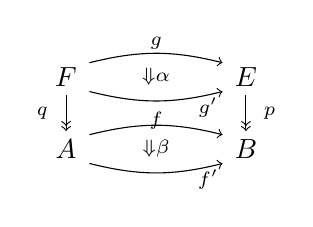
\begin{tikzpicture}[x=1.3em,y=1.3em]
  \node (F) at (0,2.0) {$F$};
  \node (E) at (5.0,2.0) {$E$};
  \node (A) at (0,0) {$A$};
  \node (B) at (5.0,0) {$B$};
  \draw[->] (0.65,2.4) to[bend left=14] (4.35,2.4);
  \node at (2.5,2.95) {$\scriptstyle g$};
  \draw[->] (0.65,1.6) to[bend right=14] (4.35,1.6);
  \node at (3.95,1.15) {$\scriptstyle g'$};
  \node at (2.5,2.0) {$\scriptstyle\Downarrow\alpha$};
  \draw[->>] (0,1.5) -- (0,0.5);
  \node at (-0.66,1.0) {$\scriptstyle q$};
  \draw[->>] (5.0,1.5) -- (5.0,0.5);
  \node at (5.66,1.0) {$\scriptstyle p$};
  \draw[->] (0.65,0.4) to[bend left=14] (4.35,0.4);
  \node at (2.5,0.8) {$\scriptstyle f$};
  \draw[->] (0.65,-0.4) to[bend right=14] (4.35,-0.4);
  \node at (3.95,-0.85) {$\scriptstyle f'$};
  \node at (2.5,0.0) {$\scriptstyle\Downarrow\beta$};
\end{tikzpicture}
\end{center}
使得 $p\alpha=\beta q$。
\end{itemize}
\end{lemma}

\begin{proof}
\cref{ex:smothering-2functor}。
\end{proof}

类似地，任何∞-宇宙都容许一个\textbf{\trTrivialFibration{}的\trInfinityCosmos}
（∞-cosmos of trivial fibrations），它可以定义为\trIsofibration{}的%
\trInfinityCosmos{}的一个全子范畴。来自抽象∞-宇宙论的下面这条一般结果解释了它
如何继承其∞-宇宙结构。

\begin{lemma}\label{lem:full-subcategory-cosmos}
设 $\mathcal{K}$ 是一个\trInfinityCosmos{}，$\mathcal{L}\subset\mathcal{K}$ 是一个
全子范畴。那么 $\mathcal{L}$ 从 $\mathcal{K}$ 继承一个由包含
$\mathcal{L}\hookrightarrow\mathcal{K}$ 创生的∞-宇宙结构，当且仅当 $\mathcal{L}$
在 $\mathcal{K}$ 中对\trCosmologicalLimitNotions{}封闭。
\end{lemma}

在实践中，我们所考虑的全子范畴都具有如下性质：$\mathcal{K}$ 中与 $\mathcal{L}$
中某个对象\trEquivalence{}的对象事实上都落在 $\mathcal{L}$ 中——换言之，这些
子范畴在定义 6.3.1 的意义下是充盈的。在下面的证明中，我们默认假定 $\mathcal{L}$
至少对同构封闭，从而一个图表的\trLimit{}只要落在 $\mathcal{L}$ 中，该图表的一切%
\trLimit{}便都落在 $\mathcal{L}$ 中；但这一假定只是为了措辞上的方便，并非本质性
的。

\begin{proof}
作为全子范畴，$\mathcal{L}$ 从 $\mathcal{K}$ 继承其\trQuasiCategory{}富集；我们
定义一个映射为 $\mathcal{L}$ 中的\trIsofibration，当且仅当它是 $\mathcal{K}$ 中的%
\trIsofibration。注意，一旦我们证明了\cref{def:infinity-cosmos}(i) 所要求的%
\trLimit{}与 $\mathcal{K}$ 中相应的\trLimit{}相重合，这一定义立即使
\cref{def:infinity-cosmos}(ii) 得到满足。而这恰恰就是「$\mathcal{L}$ 在
$\mathcal{K}$ 中对\trCosmologicalLimitNotions{}封闭」这一假设所断言的。

我们已经证明：一个封闭的全子范畴以一种使包含 $\mathcal{L}\hookrightarrow\mathcal{K}$
成为反射\trIsofibration{}与\trCosmologicalLimitNotions{}的%
\trCosmologicalFunctor{}的方式继承一个∞-宇宙结构。显然，这一包含反射可表示地
定义的\trEquivalence，因为
$\mathcal{L}$ 是 $\mathcal{K}$ 的全子范畴。但由引理 1.3.2，\trCosmologicalFunctor{}
$\mathcal{L}\hookrightarrow\mathcal{K}$ 也保持它们，这告诉我们：$\mathcal{L}$ 中的%
\trEquivalence{}随\trIsofibration{}与\trCosmologicalLimitNotions{}一道，从
$\mathcal{K}$ 创生而来。
\end{proof}

有了这一结果，进一步的∞-宇宙便不难确立了。

\begin{proposition}[平凡纤维化的∞-宇宙]\label{prop:trivial-fibration-cosmoi}
设 $\mathcal{K}$ 是一个\trInfinityCosmos。
\begin{itemize}
\item[(i)] 对 $\mathcal{K}$ 中任何\trInfinityCategory{} $B$，由余定义域为 $B$
的那些\trTrivialFibration{}张成的全子范畴
$\mathcal{K}^{\approx}_{/B}\hookrightarrow\mathcal{K}_{/B}$
定义一个∞-宇宙，其\trLimit、\trIsofibration、\trEquivalence{}与%
\trTrivialFibration{}均由包含函子创生。
\item[(ii)] 由\trTrivialFibration{}张成的全子范畴
$\mathcal{K}^{\natural}\hookrightarrow\mathcal{K}^{\dagger}$
定义一个∞-宇宙，其\trLimit、\trIsofibration、\trEquivalence{}与%
\trTrivialFibration{}均由包含函子创生。
\end{itemize}
\end{proposition}

\begin{proof}
其细节与命题 1.2.22 及\cref{prop:isofibration-cosmos}类似，留作%
\cref{ex:trivial-fibration-cosmoi}。
\end{proof}

注意，平凡纤维化的诸\trSliceInfinityCosmos{} $\mathcal{K}^{\approx}_{/B}$ 是弱可缩的，其意义
是：到\trTerminal{}∞-宇宙 $\qcOne$ 的唯一\trFunctor{}
$\mathcal{K}^{\approx}_{/B}\rightsquigarrow\qcOne$ 是一个%
\trCosmologicalBiequivalence。特别地，$\mathcal{K}^{\approx}_{/B}$ 中的每个%
\trFunctor{}都是\trEquivalence，因此这个∞-宇宙与其说是一个有实质意义的结构，
不如说是一件奇物。

正如 1.2 节中所许诺的，\cref{lem:full-subcategory-cosmos}使我们能够推广命题
1.2.12，以证明任何∞-宇宙中的\trDiscrete{}\trInfinityCategory{}构成一个∞-宇宙：

\begin{proposition}[离散∞-范畴的∞-宇宙]\label{prop:discrete-cosmos}
任何\trInfinityCosmos{}中由\trDiscrete{}\trInfinityCategory{}张成的全子范畴
$\mathcal{K}^{\approx}\hookrightarrow\mathcal{K}$ 继承一个由包含创生的∞-宇宙
结构。
\end{proposition}

\begin{proof}
回忆引理 1.2.27：∞-宇宙 $\mathcal{K}$ 中的一个\trInfinityCategory{} $E$ 是离散
的，当且仅当映射 $E^{\qcOne}\twoheadrightarrow E^{\qcTwo}$ 是\trTrivialFibration。
这表明，由\trDiscrete{}\trInfinityCategory{}组成的全子范畴
$\mathcal{K}^{\approx}\hookrightarrow\mathcal{K}$ 由沿\trCosmologicalFunctor{}
$I$ 的如下\trPullback{}定义——$I$ 把一个\trInfinityCategory{} $E$ 送到%
\trIsofibration{} $E^{\qcOne}\twoheadrightarrow E^{\qcTwo}$：
\begin{center}
\begin{tikzpicture}[x=1.3em,y=1.3em]
  \node (TL) at (0,1.7) {$\mathcal{K}^{\approx}$};
  \node (TR) at (5.2,1.7) {$\mathcal{K}^{\natural}$};
  \node (BL) at (0,0) {$\mathcal{K}$};
  \node (BR) at (5.2,0) {$\mathcal{K}^{\dagger}$};
  \draw[->] (0.85,1.7) -- (4.15,1.7);
  \draw[right hook->] (0,1.2) -- (0,0.5);
  \node at (0.5,1.28) {$\scriptstyle\lrcorner$};
  \draw[right hook->] (5.2,1.2) -- (5.2,0.5);
  \draw[->] (0.85,0) -- node[below]{$\scriptstyle I$} (4.15,0);
\end{tikzpicture}
\end{center}
由\cref{lem:full-subcategory-cosmos}，为证明 $\mathcal{K}^{\approx}$ 容许一个从
$\mathcal{K}$ 继承的∞-宇宙结构，我们只需证明离散∞-范畴在 $\mathcal{K}$ 中对
\cref{def:infinity-cosmos}(i) 的诸极限构造封闭。以单纯余张量为例，这可以很容易地
从其定义泛性质以及\trKanComplex{}构成\trSimplicialSet{}范畴的一个%
\trExponentialIdeal{}这一事实推出。对每个锥形\trLimit{}都可以给出一个共同的
论证；为具体起见，考虑离散∞-范畴之间由\trIsofibration{}构成的一座塔 $E_{n}$，
并在 $\mathcal{K}$ 中取其\trLimit
\begin{equation*}
E:=\lim\Big(\ \cdots\twoheadrightarrow E_{n}\twoheadrightarrow E_{n-1}
\twoheadrightarrow\cdots\twoheadrightarrow E_{1}\twoheadrightarrow E_{0}\ \Big).
\end{equation*}
\trCosmologicalFunctor{} $I$ 把它送到∞-宇宙 $\mathcal{K}^{\dagger}$ 中的一个%
\trLimit{}图表
\begin{equation*}
\begin{array}{c}
E^{\qcOne}\\[0.1em]
\twoheaddownarrow\\[0.1em]
E^{\qcTwo}
\end{array}
:=\lim\left(\begin{array}{ccccccccccc}
\cdots&\twoheadrightarrow&E_{n}^{\qcOne}&\twoheadrightarrow&E_{n-1}^{\qcOne}
 &\twoheadrightarrow&\cdots&\twoheadrightarrow&E_{1}^{\qcOne}
 &\twoheadrightarrow&E_{0}^{\qcOne}\\
&&\twoheaddownarrow&&\twoheaddownarrow&&&&\twoheaddownarrow&&\twoheaddownarrow\\
\cdots&\twoheadrightarrow&E_{n}^{\qcTwo}&\twoheadrightarrow&E_{n-1}^{\qcTwo}
 &\twoheadrightarrow&\cdots&\twoheadrightarrow&E_{1}^{\qcTwo}
 &\twoheadrightarrow&E_{0}^{\qcTwo}
\end{array}\right).
\end{equation*}
由于每个 $E_{n}$ 都是\trDiscrete{}\trInfinityCategory，此图表中的每个对象都是%
\trTrivialFibration。于是，由\cref{prop:trivial-fibration-cosmoi}，这个\trLimit{}
$E^{\qcOne}\twoheadrightarrow E^{\qcTwo}$ 也是\trTrivialFibration。这就证明了 $E$ 是
离散的。
\end{proof}

\cref{prop:isofibration-cosmos}的证明表明，在构造新\trInfinityCosmos{}时以手工
验证极限公理是件繁琐的事情；的确，即便在那个相对基本的例子中，我们也略去了一些
细节。在接下来的几节中，我们将发展一套机制，使我们能够更系统地攻克这一问题。

\subsection*{练习}

\begin{exercise}\label{ex:smothering-2functor}
证明\cref{lem:smothering-2functor}。
\end{exercise}

\begin{exercise}\label{ex:trivial-fibration-cosmoi}
用\cref{lem:full-subcategory-cosmos}证明\cref{prop:trivial-fibration-cosmoi}。
\end{exercise}

\begin{exercise}\label{ex:inverse-reedy-cosmos}
设 $\mathcal{K}$ 是一个\trInfinityCosmos{}，$\mathcal{J}$ 是一个\emph{逆范畴}
（inverse category）（见定义 C.1.16）。在命题 C.1.23 的指引下，证明存在一个%
\trInfinityCosmos{} $\mathcal{K}^{\mathcal{J}}$，使得：
\begin{itemize}
\item 其对象是定义 C.1.19 的\emph{\trFibrant{}图表}；
\item 其\trIsofibration{}是定义 C.1.19 的\emph{\trFibrant{}自然变换}；
\item 其\trFunctorSpace{}是定义 A.3.8 的单纯 hom-空间；
\item 且其中的单纯\trLimit{}与\trEquivalence{}在 $\mathcal{K}$ 中逐点定义。
\end{itemize}
用命题 C.1.21 证明：\trFibrant{} $\mathcal{J}$-索引图表之\trLimit{}在
$\mathcal{K}$ 中存在，并且\trFunctor{}
$\lim\colon\mathcal{K}^{\mathcal{J}}\to\mathcal{K}$ 是宇宙论的。
\end{exercise}
